\PassOptionsToPackage{table, dvipsnames}{xcolor}
\documentclass[11pt]{beamer} %%

%%% option passed to the outer theme
% fixedCircCnt,   % (moving is deault)
\usetheme[progressstyle=movingCircCnt]{Feather}


%%xcolor=dvipsnames,
%-------------------------------------------------------
% INCLUDE PACKAGES
%-------------------------------------------------------

\usepackage[utf8]{inputenc} 
\usepackage[english]{babel}

\usepackage{wrapfig}
\usepackage{graphicx}
\usepackage{tikz}
\usetikzlibrary{decorations.fractals, spy, intersections, calc}

\usepackage{braket}

\usepackage{mathpazo} 
\usepackage{amsmath, amsthm, amssymb}

\usepackage{amsfonts}
%\usepackage{mathrsfs}
\usepackage{slashed} % Dirac slash
\usepackage{pifont}
\usepackage{caption}

%%%% multimedia
%%\usepackage{multimedia}
%%\usepackage{hyperref}


%%%% fonts
\usepackage{tgtermes}
%% change font of the document 
%\renewcommand*{\familydefault }{\mrdefault}
\usefonttheme{professionalfonts} % using non standard fonts for beamer
\usefonttheme{serif} % default family is serif
\usepackage{fontspec}
\setmainfont{Latin Modern Roman}

%%%% colors
% Change the frame title text color:
\setbeamercolor{frametitle}{fg=BurntOrange}
% Change the normal text color background:
\setbeamercolor{normal text}{fg=black,bg=white}
%%% color equations 
\usepackage[skins,theorems]{tcolorbox}
\tcbset{highlight math style={enhanced,
  colframe=red,colback=white,arc=0pt,boxrule=1pt}}

%%%% colourful equation box
\tcbset{highlight math style={enhanced,
  colframe=red,colback=white,arc=0pt,boxrule=1pt}}
\newcommand{\eqbox}[3]
           {
             \tcbhighmath[boxrule=2pt,arc=1pt,colback=#1!10!white,colframe=#2!40,
               drop fuzzy shadow=white] {#3}
           }

%%%%  tables
%%\usepackage[landscape]{geometry}
\usepackage{multirow}
\usepackage{changepage}
\usepackage{longtable}
\usepackage{booktabs}

%% for pdf input
\usepackage{pdfpages}
\usepackage{forloop}

%%%% set footers
\setbeamertemplate{footline}[text line]{%
  \parbox{0.3\linewidth}{\vspace*{-5pt}\hspace*{0.5cm}
    \textcolor{BurntOrange}{{-- D$\emptyset$ Detector}}}\hfill
  \parbox{0.4\linewidth}{\vspace*{-5pt}\hspace*{1.cm}
    \textcolor{BurntOrange}{{ -- Sina Bahrasemani --}}}\hfill
  \parbox{0.3\linewidth}{\vspace*{-5pt}\hspace*{1.5cm}
    \textcolor{BurntOrange}{{Fall 2017 --}}}\hfill
}
%%\setbeamertemplate{footline}[page number]

% colored hyperlinks
\newcommand{\chref}[2]
           {
             \href{#1}{{\usebeamercolor[bg]{Feather}#2}}
           }

%%%% few extra commands
\renewcommand{\(}{\begin{columns}}
\renewcommand{\)}{\end{columns}}
\newcommand{\<}[1]{\begin{column}{#1}}
\renewcommand{\>}{\end{column}}

\newcommand{\itt}{\begin{itemize}}
\newcommand{\tti}{\end{itemize}}

\newcommand{\img}[1]{\includegraphics[width=\linewidth]{./Images/#1}}

\newcommand{\hlt}[2]{\textcolor{#1}{\textbf{#2}}}
\newcommand{\ntit}[1]{\qquad\qquad\qquad\qquad\hlt{blue}{\Large #1}\\~\\}
%% \newcommand{\hlt1}[1]{\textcolor{Goldenrod}{\textbf{#1}}}
\newcommand{\cmark}{\ding{51}}%
\newcommand{\done}
           {
             \rlap{$\square$}
                  {\raisebox{2pt}
                    {
                      \large\hspace{0.1pt}
                      \textcolor{green}{\cmark}
                    }
                  }
                  \hspace{-2.5pt}
           }

           
%%% counting backup slides
\newcommand{\beginbackup}
           {
             \newcounter{framenumbervorappendix}
             \setcounter{framenumbervorappendix}{\value{framenumber}}
           }
\newcommand{\backupend}
           {
             \addtocounter{framenumbervorappendix}{-\value{framenumber}}
             \addtocounter{framenumber}{\value{framenumbervorappendix}} 
           }

%%%% Loading packages DONE!
%\logo{
\includegraphics[scale = 0.2]{./Images/SFU_logo.jpg}}


%%%% user libs 
\usepackage{graphicx}
\usepackage{caption}
\usepackage{subcaption}
\usepackage{tikz}
\usepackage{pgfplots}
\usetikzlibrary{spy,calc}
\usepackage{hyperref}


\newif\ifblackandwhitecycle
\gdef\patternnumber{0}

\pgfkeys{/tikz/.cd,
    zoombox paths/.style={
        draw=orange,
        very thick
    },
    black and white/.is choice,
    black and white/.default=static,
    black and white/static/.style={ 
        draw=white,   
        zoombox paths/.append style={
            draw=white,
            postaction={
                draw=black,
                loosely dashed
            }
        }
    },
    black and white/static/.code={
        \gdef\patternnumber{1}
    },
    black and white/cycle/.code={
        \blackandwhitecycletrue
        \gdef\patternnumber{1}
    },
    black and white pattern/.is choice,
    black and white pattern/0/.style={},
    black and white pattern/1/.style={    
            draw=white,
            postaction={
                draw=black,
                dash pattern=on 2pt off 2pt
            }
    },
    black and white pattern/2/.style={    
            draw=white,
            postaction={
                draw=black,
                dash pattern=on 4pt off 4pt
            }
    },
    black and white pattern/3/.style={    
            draw=white,
            postaction={
                draw=black,
                dash pattern=on 4pt off 4pt on 1pt off 4pt
            }
    },
    black and white pattern/4/.style={    
            draw=white,
            postaction={
                draw=black,
                dash pattern=on 4pt off 2pt on 2 pt off 2pt on 2 pt off 2pt
            }
    },
    zoomboxarray inner gap/.initial=5pt,
    zoomboxarray columns/.initial=2,
    zoomboxarray rows/.initial=2,
    subfigurename/.initial={},
    figurename/.initial={zoombox},
    zoomboxarray/.style={
        execute at begin picture={
            \begin{scope}[
                spy using outlines={%
                    zoombox paths,
                    width=\imagewidth / \pgfkeysvalueof{/tikz/zoomboxarray columns} - (\pgfkeysvalueof{/tikz/zoomboxarray columns} - 1) / \pgfkeysvalueof{/tikz/zoomboxarray columns} * \pgfkeysvalueof{/tikz/zoomboxarray inner gap} -\pgflinewidth,
                    height=\imageheight / \pgfkeysvalueof{/tikz/zoomboxarray rows} - (\pgfkeysvalueof{/tikz/zoomboxarray rows} - 1) / \pgfkeysvalueof{/tikz/zoomboxarray rows} * \pgfkeysvalueof{/tikz/zoomboxarray inner gap}-\pgflinewidth,
                    magnification=3,
                    every spy on node/.style={
                        zoombox paths
                    },
                    every spy in node/.style={
                        zoombox paths
                    }
                }
            ]
        },
        execute at end picture={
            \end{scope}
            \node at (image.north) [anchor=north,inner sep=0pt] {\subcaptionbox{\label{\pgfkeysvalueof{/tikz/figurename}-image}}{\phantomimage}};
            \node at (zoomboxes container.north) [anchor=north,inner sep=0pt] {\subcaptionbox{\label{\pgfkeysvalueof{/tikz/figurename}-zoom}}{\phantomimage}};
     \gdef\patternnumber{0}
        },
        spymargin/.initial=0.5em,
        zoomboxes xshift/.initial=1,
        zoomboxes right/.code=\pgfkeys{/tikz/zoomboxes xshift=1},
        zoomboxes left/.code=\pgfkeys{/tikz/zoomboxes xshift=-1},
        zoomboxes yshift/.initial=0,
        zoomboxes above/.code={
            \pgfkeys{/tikz/zoomboxes yshift=1},
            \pgfkeys{/tikz/zoomboxes xshift=0}
        },
        zoomboxes below/.code={
            \pgfkeys{/tikz/zoomboxes yshift=-1},
            \pgfkeys{/tikz/zoomboxes xshift=0}
        },
        caption margin/.initial=4ex,
    },
    adjust caption spacing/.code={},
    image container/.style={
        inner sep=0pt,
        at=(image.north),
        anchor=north,
        adjust caption spacing
    },
    zoomboxes container/.style={
        inner sep=0pt,
        at=(image.north),
        anchor=north,
        name=zoomboxes container,
        xshift=\pgfkeysvalueof{/tikz/zoomboxes xshift}*(\imagewidth+\pgfkeysvalueof{/tikz/spymargin}),
        yshift=\pgfkeysvalueof{/tikz/zoomboxes yshift}*(\imageheight+\pgfkeysvalueof{/tikz/spymargin}+\pgfkeysvalueof{/tikz/caption margin}),
        adjust caption spacing
    },
    calculate dimensions/.code={
        \pgfpointdiff{\pgfpointanchor{image}{south west} }{\pgfpointanchor{image}{north east} }
        \pgfgetlastxy{\imagewidth}{\imageheight}
        \global\let\imagewidth=\imagewidth
        \global\let\imageheight=\imageheight
        \gdef\columncount{1}
        \gdef\rowcount{1}
        \gdef\zoomboxcount{1}
    },
    image node/.style={
        inner sep=0pt,
        name=image,
        anchor=south west,
        append after command={
            [calculate dimensions]
            node [image container,subfigurename=\pgfkeysvalueof{/tikz/figurename}-image] {\phantomimage}
            node [zoomboxes container,subfigurename=\pgfkeysvalueof{/tikz/figurename}-zoom] {\phantomimage}
        }
    },
    color code/.style={
        zoombox paths/.append style={draw=#1}
    },
    connect zoomboxes/.style={
    spy connection path={\draw[draw=none,zoombox paths] (tikzspyonnode) -- (tikzspyinnode);}
    },
    help grid code/.code={
        \begin{scope}[
                x={(image.south east)},
                y={(image.north west)},
                font=\footnotesize,
                help lines,
                overlay
            ]
            \foreach \x in {0,1,...,9} { 
                \draw(\x/10,0) -- (\x/10,1);
                \node [anchor=north] at (\x/10,0) {0.\x};
            }
            \foreach \y in {0,1,...,9} {
                \draw(0,\y/10) -- (1,\y/10);                        \node [anchor=east] at (0,\y/10) {0.\y};
            }
        \end{scope}    
    },
    help grid/.style={
        append after command={
            [help grid code]
        }
    },
}

\newcommand\phantomimage{%
    \phantom{%
        \rule{\imagewidth}{\imageheight}%
    }%
}
\newcommand\zoombox[2][]{
    \begin{scope}[zoombox paths]
        \pgfmathsetmacro\xpos{
            (\columncount-1)*(\imagewidth / \pgfkeysvalueof{/tikz/zoomboxarray columns} + \pgfkeysvalueof{/tikz/zoomboxarray inner gap} / \pgfkeysvalueof{/tikz/zoomboxarray columns} ) + \pgflinewidth
        }
        \pgfmathsetmacro\ypos{
            (\rowcount-1)*( \imageheight / \pgfkeysvalueof{/tikz/zoomboxarray rows} + \pgfkeysvalueof{/tikz/zoomboxarray inner gap} / \pgfkeysvalueof{/tikz/zoomboxarray rows} ) + 0.5*\pgflinewidth
        }
        \edef\dospy{\noexpand\spy [
            #1,
            zoombox paths/.append style={
                black and white pattern=\patternnumber
            },
            every spy on node/.append style={#1},
            x=\imagewidth,
            y=\imageheight
        ] on (#2) in node [anchor=north west] at ($(zoomboxes container.north west)+(\xpos pt,-\ypos pt)$);}
        \dospy
        \pgfmathtruncatemacro\pgfmathresult{ifthenelse(\columncount==\pgfkeysvalueof{/tikz/zoomboxarray columns},\rowcount+1,\rowcount)}
        \global\let\rowcount=\pgfmathresult
        \pgfmathtruncatemacro\pgfmathresult{ifthenelse(\columncount==\pgfkeysvalueof{/tikz/zoomboxarray columns},1,\columncount+1)}
        \global\let\columncount=\pgfmathresult
        \ifblackandwhitecycle
            \pgfmathtruncatemacro{\newpatternnumber}{\patternnumber+1}
            \global\edef\patternnumber{\newpatternnumber}
        \fi
    \end{scope}
}



%%%%%%%%%%%%%%%%%%%%%%%%%%%%%%%%%%%%%%%%%%%%%%%%%%%%%%%%%%%%%%%%%%%%%%%%%%%%%%%%%%%%%%%
%%%%%%%%%%%%%%%% DOCUMENT STARTS HERE
\begin{document}
\setbeamercovered{transparent}

%%%% SLIDE 1: title page
\begin{frame}
	\vspace{0.9cm}

\title[]{D$\emptyset$ Detector}
\author{Sina Bahrasemani\\
  \vspace{0.2in}
}
\date{
  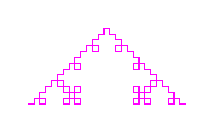
\begin{tikzpicture}[decoration=Koch curve type 1] 
    \draw[Magenta] decorate{ decorate{ decorate{ (0,0) -- (2,0) }}}; 
  \end{tikzpicture}  
  \\
  \vspace{0.2cm}
  \today
}
\titlepage
\end{frame}

%%%%%%%% SLIDE 2: outline page
\begin{frame}{Outline}
\small
\tableofcontents[hideallsubsections]

\end{frame}

%%%%%%% LOAD section files here
% % % \section{D$\emptyset$ detector}
% % % \section{Central detector}
% % % \section{Solenoidal magnet}
% % % \section{Preshower detectors}
% % % \section{Calorimetry}
% % % \section{Muon system}
% % % \section{Forward proton detector}
% % % \section{Luminosity monitor}
% % % \section{Triggering}

\foreach \index in {1, ..., 7}{
  \input{section0\index.tex}\par
}


%%%%%%%%%%%%%% APPENDIX
\newcounter{finalframe}
\setcounter{finalframe}{\value{framenumber}}
\beginbackup
%\usebackgroundtemplate{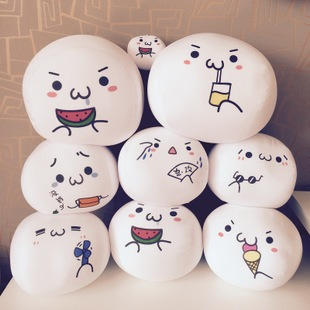
\includegraphics[width=\textwidth]{./Images/200_thank_you_01}}
\begin{frame}[noframenumbering]
  \hlt{ForestGreen}{Thank you }
\end{frame}


\section*{Appendix}


%%%%%%%%%%%%%%%%%%%%%%%%%%%%%%%%%%%%%%%%%%%%
\subsection*{D$\emptyset$ Goals}
%%%%% SLIDE
\begin{frame}{\textcolor{Goldenrod}{D$\emptyset$ Experiment Goals}}

  \itt[<only@+>]
\item[$\Box$] \hlt{black}{Z and W masses:\\}
  $-$ Z mass from $ Z\to e^+ e^-$ using invariant mass\\
  $-$ W mass from $W\to l \nu_{l}$ using $m_{T} =
  \sqrt{2p^{l}_{T}\slashed{E_{T}}(1 - \cos\theta_{l, MET})}$\\
  $-$ good $\slashed{E_{T}}$ resolution is necessary for $m_T$
\item[$\Box$] \hlt{black}{Z and W widths:}\\
  $- $ \alert{$\delta \Gamma_Z = \frac{2}{N} \sqrt{\Gamma^2_Z + (2.35
      \delta m_Z)^2}$}\\
  $- $ $\frac{\Gamma_W}{\Gamma_Z}$ within 8\% $\to$ QCD radiative
  corrections  \& narrowing down $m_t$ mass window

\item[$\Box$] \hlt{black}{$Z \to X \gamma; X\to l^+l^-$ searches:} \\
  $- $ electronic to muonic decay ratio is needed\\
  $- $ \alert{ good $\gamma$ ( ~ 10 GeV) and $\pi^0$ separation is
    essential}
  
\item[$\Box$] \hlt{black}{ Forward-backward asymmetry:}\\
  $- $ $b\bar{b}$ decay was of special interest due to pure measurements
  from other experiments\\
  $- $ good muon identification at $p_T \approx 100 GeV/c$
  
%% 03_tri_couplings  
\item  \hlt{black}{Gauge boson couplings:\\}
  $- $ associated production of gauge bosons
  $- $ $p\bar{p} \to W \gamma X; W \to l \nu$ 

\item \hlt{black}{ W and Z production:}\\
  $- $ The x-dependence of W and Z production reveal the parton
  x-distribution in the same way as in Drell-Yan production.\\
  
  $- $ The $p_T$ distribution of produced bosons is interesting for a
  study of radiative processes in QCD

\item \hlt{black}{$W/Z \to q\bar{q}$:}\\
  $- $ good hadron energy measurement in order to reduce the error on jet
  invariant mass.\\
  $- $ good segmentation of calorimetry is also desired
  
\item \hlt{black}{ $\frac{\alpha_{QCD}}{\alpha_{QED}}$ :\\} 
  $- $ single $\gamma$ to single $g$ production 
  \tti
  
\end{frame}


%%%%%%%% SLIDE
\begin{frame}{\textcolor{Goldenrod}{D$\emptyset$ Design Considerations}}
  \itt
\item[$\bullet$]
  \textcolor{blue}{Electromagnetic energy resolution at the level of $\delta E / E
    = \frac{0.05}{\sqrt{E}}$ with good $\pi^0-e $ separation}
  {\small
    \itt
  \item good electron ID for narrow massive states searches and
    to lower electron-jet faking rate. \\
  \item good lateral and longitudinal sampling for single $\gamma$
    searches with high $p_T$ (\alert{challenging $\pi^0-e $ separation})
    \tti
  }
  
\item[$\bullet$]
  \textcolor{blue}{good muon momentum resolution and
    muon ID}
  {\small
    \itt
  \item muons are less analyzed, but with charge tagging $\to$ ID them even inside
    jets which is important for many searches
    \tti
  }
  \tti
\end{frame}


%%%%%%% SLIDE 
\begin{frame}{\textcolor{Goldenrod}{Upgraded D$\emptyset$ }}
  % \<{0.5\textwidth}
  % \begin{center}
  %   \img{01_dzero_wholedetector}
  % \end{center}
  % % \caption*{{\scriptsize A simplified cross section view of the
  % % D$\emptyset$   }}
  % \>
  \itt
\item[$\Box$]<only@1> \hlt{Blue}{in 2001 after the Main Injector and associated Tevatron
  upgrades the instantaneous luminosity increased by more than a factor of ten}
  
\item[$\Box$]<only@1> \hlt{Magenta}{The central tracking system was completely replaced.}
  {\small
    \itt
  \item \alert{the old system lacked a magnetic field and suffered from radiation
      damage}
  \item improved tracking technologies are now available.\\
  \item The new system included a silicon microstrip tracker and a
    scintillating-fiber tracker located within a 2 T solenoidal
    magnet.
    \tti
  }
\item[$\Box$]<only@2> \hlt{blue}{Between the solenoidal magnet and the central calorimeter and
    in front of the forward calorimeters, preshower detectors have
    been added for improved electron identification.}
  
\item[$\Box$]<only@2> \hlt{blue}{In the forward muon system, proportional drift chambers are
    replaced by mini drift tubes and trigger scintillation
    counters\\}
  {\small
    \itt
  \item which can withstand the harsh radiation environment and
    additional shielding has been added.
    
  \item \alert{In the central region,
      scintillation counters have been added for improved muon
      triggering.}
    \tti
  }
  \tti
\end{frame}


%%%%%%% SLIDE
\begin{frame}{\textcolor{Goldenrod}{p-n Junction}}
  \begin{figure}[h]\centering
    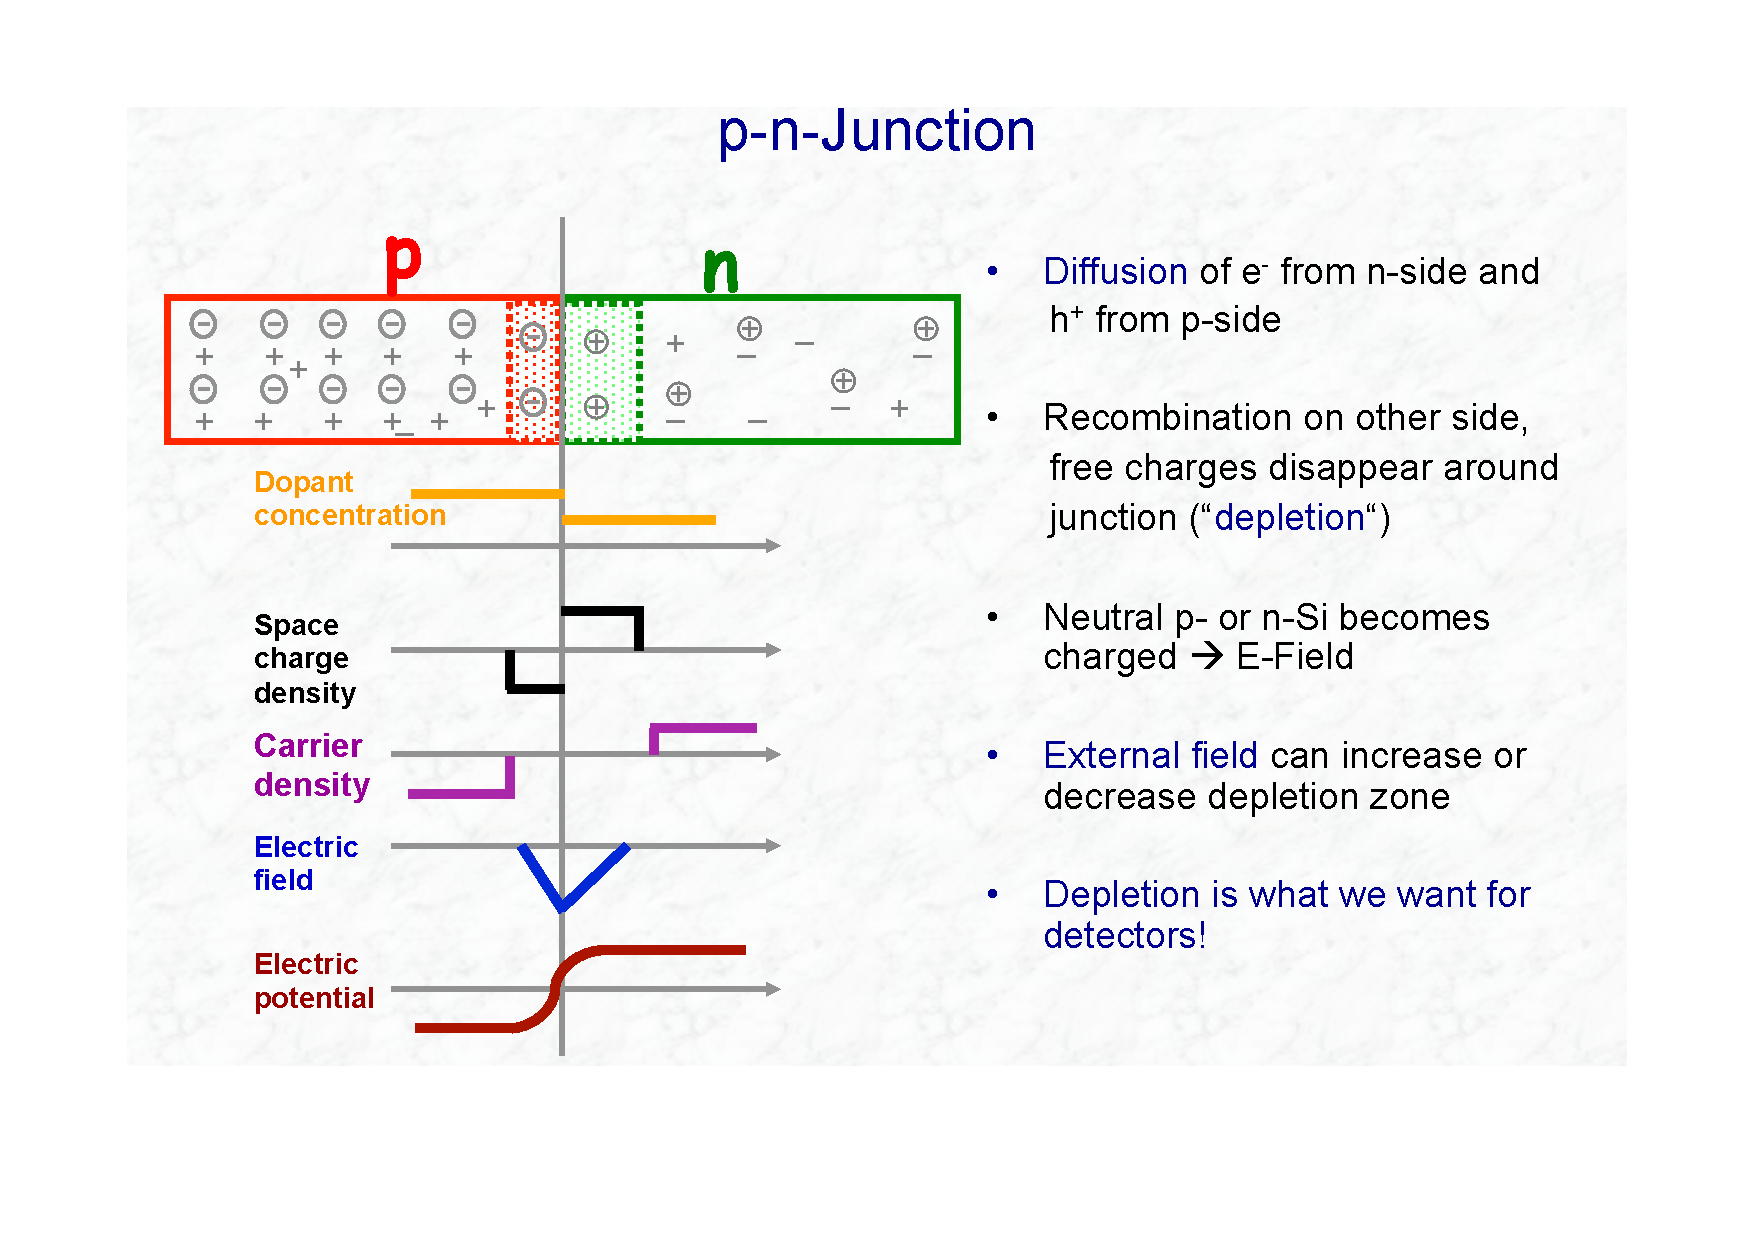
\includegraphics[width=0.95\linewidth]{./Images/104_extra_pn_junction}
  \end{figure}
\end{frame}

%%%%%%% SLIDE
\begin{frame}{\textcolor{Goldenrod}{Basic Silicon Detector}}
  \begin{figure}[h]\centering
    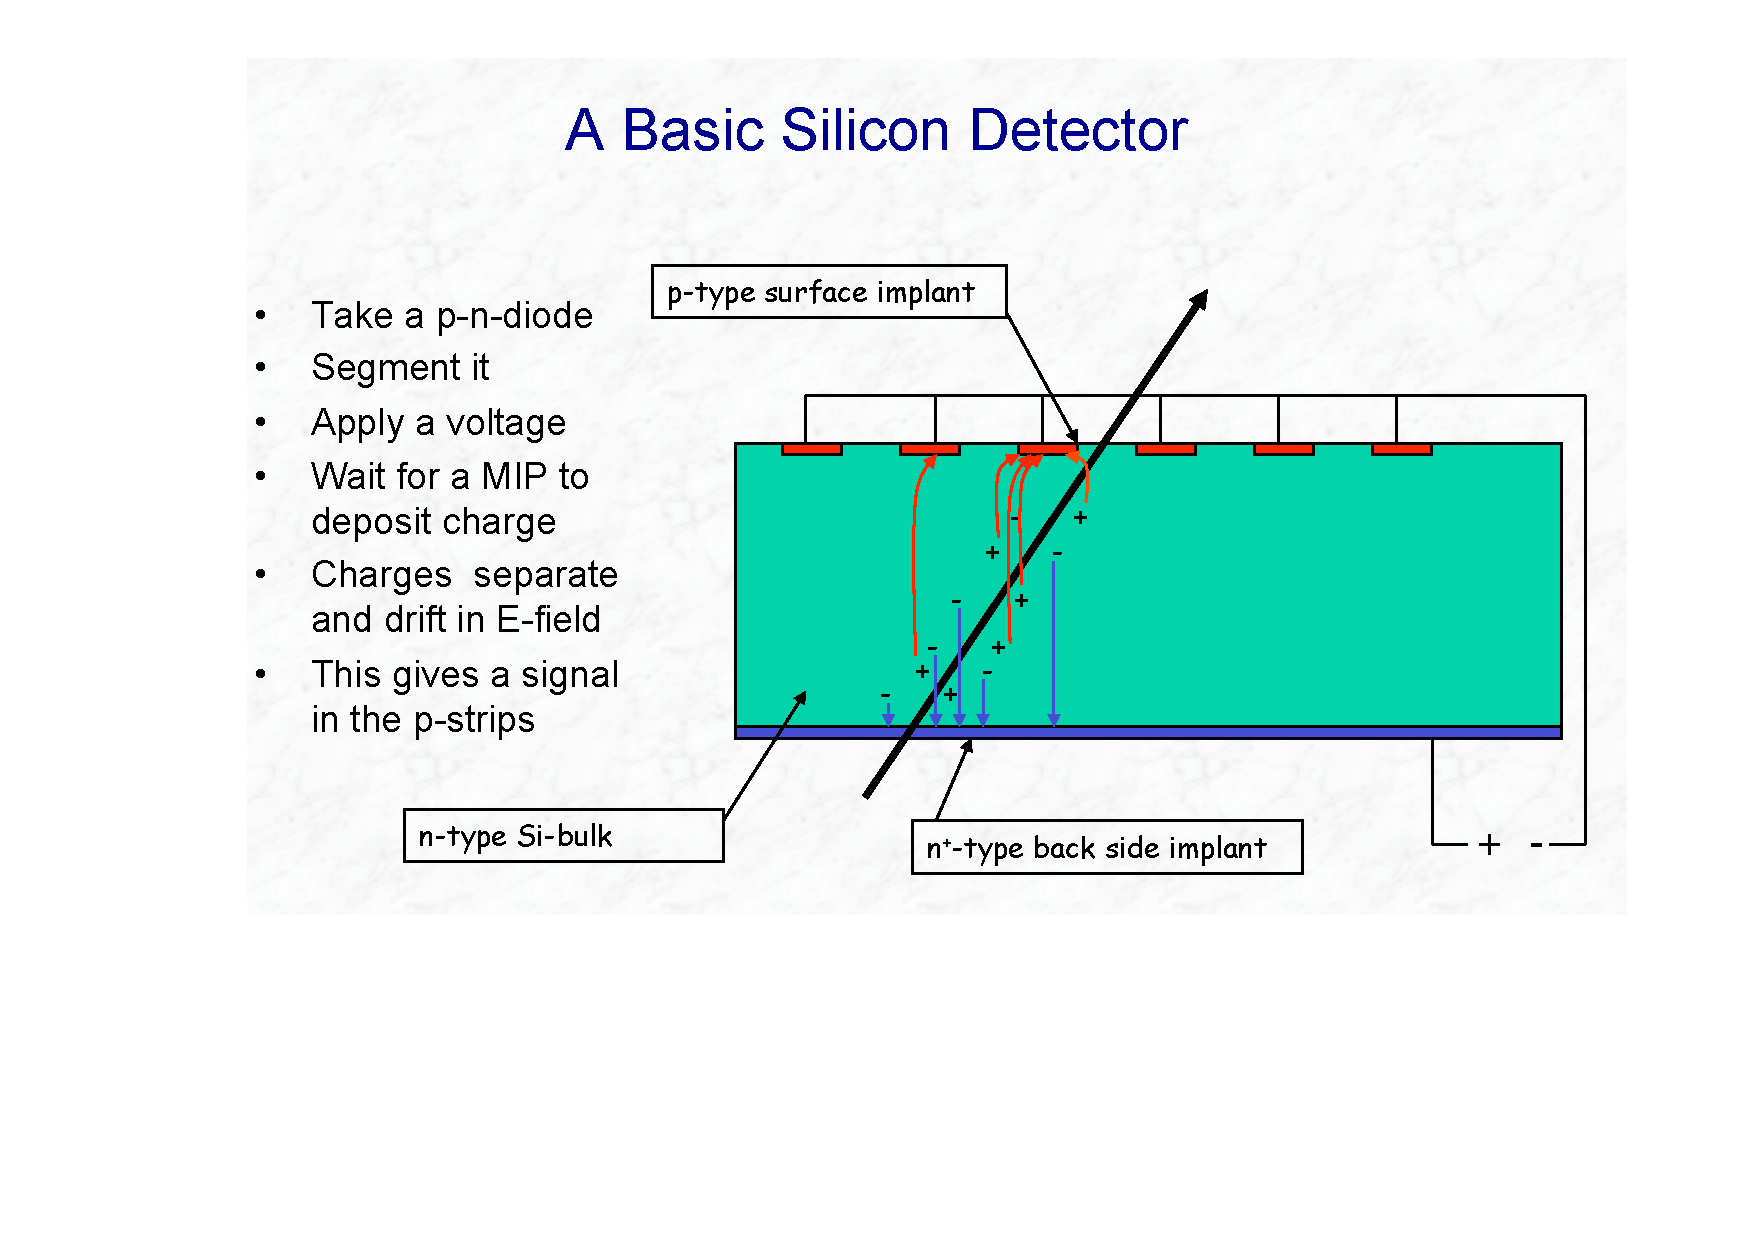
\includegraphics[width=0.95\linewidth]{./Images/105_extra_silicon_detector}
  \end{figure}
\end{frame}


%%%%%%% SLIDE
\begin{frame}{\textcolor{Goldenrod}{DSDM Silicon Detector}}
  \begin{figure}[h]\centering
    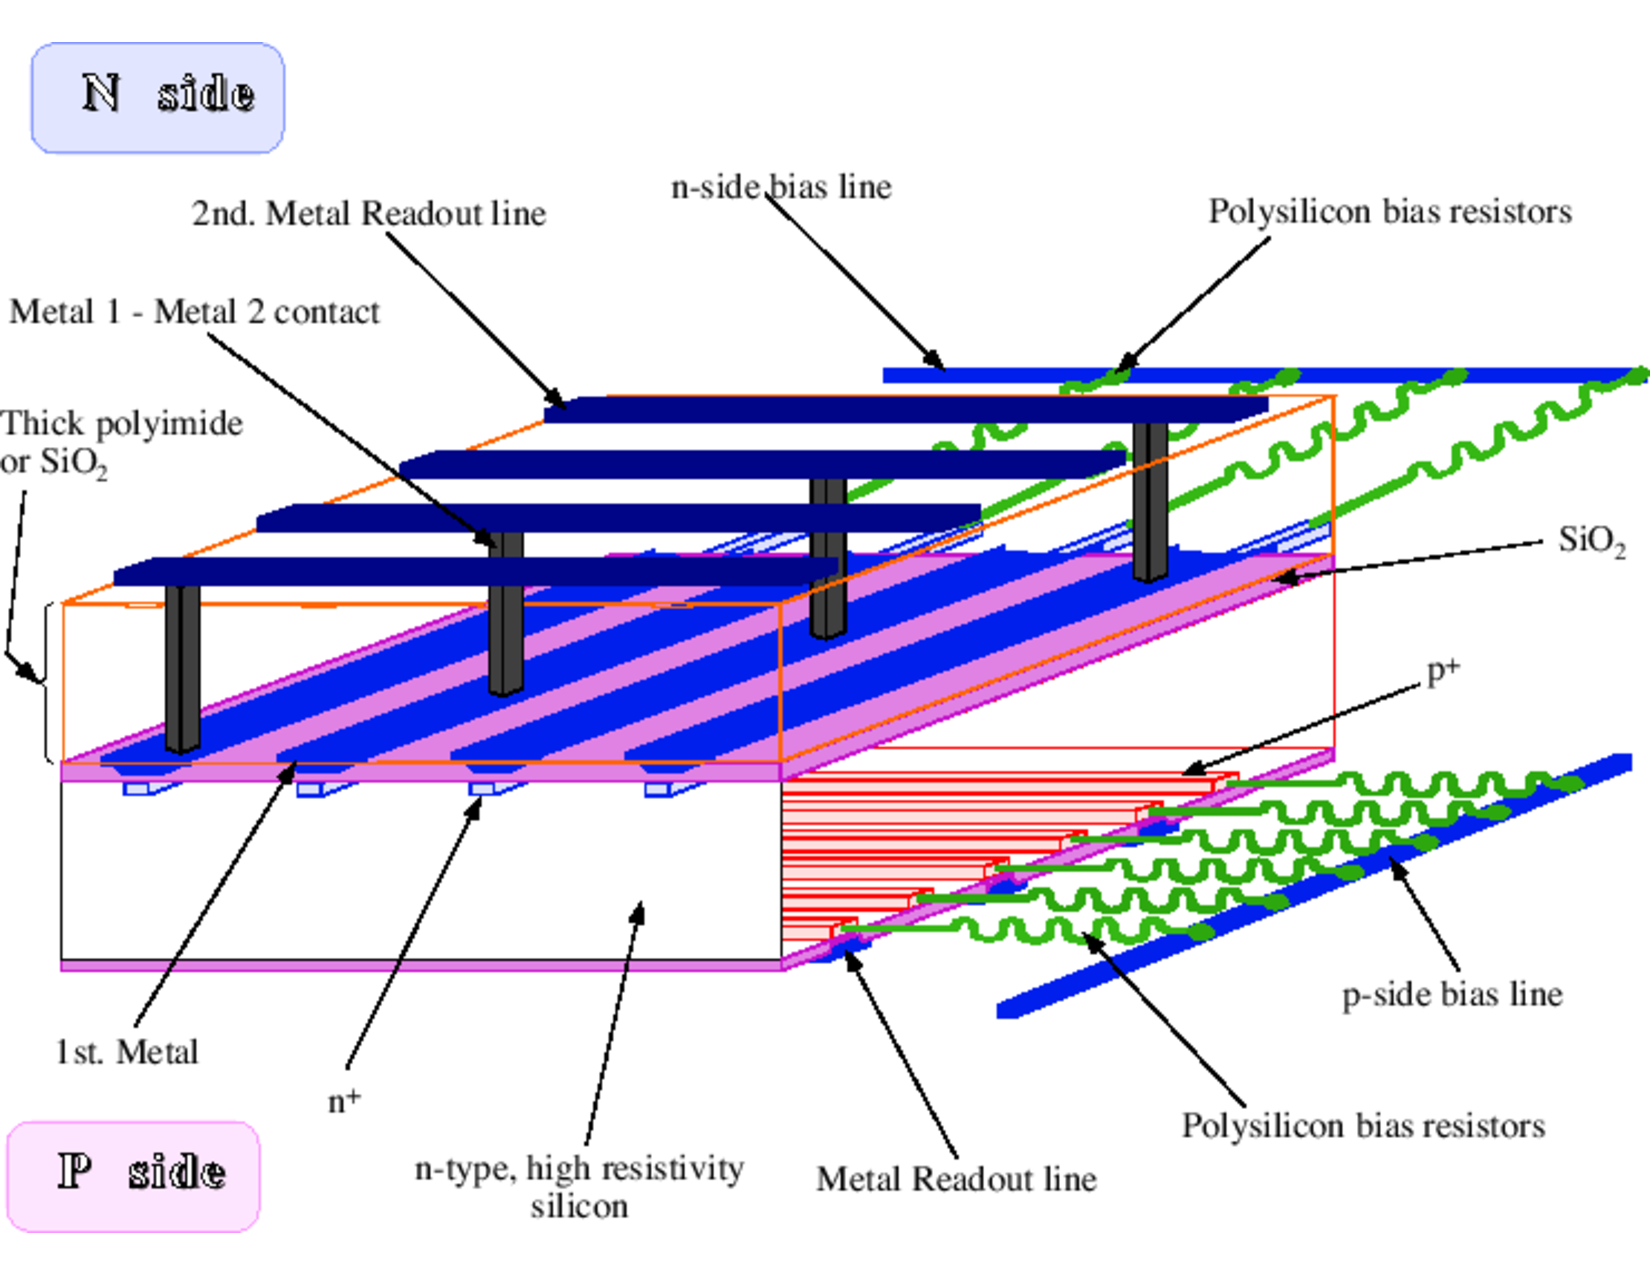
\includegraphics[width=0.95\linewidth]{./Images/106_extra_DSDM.pdf}
  \end{figure}
\end{frame}


%%%%%%% SLIDE
\begin{frame}{\textcolor{Goldenrod}{Visible Light Photon Counters}}
  \begin{figure}[h]\centering
    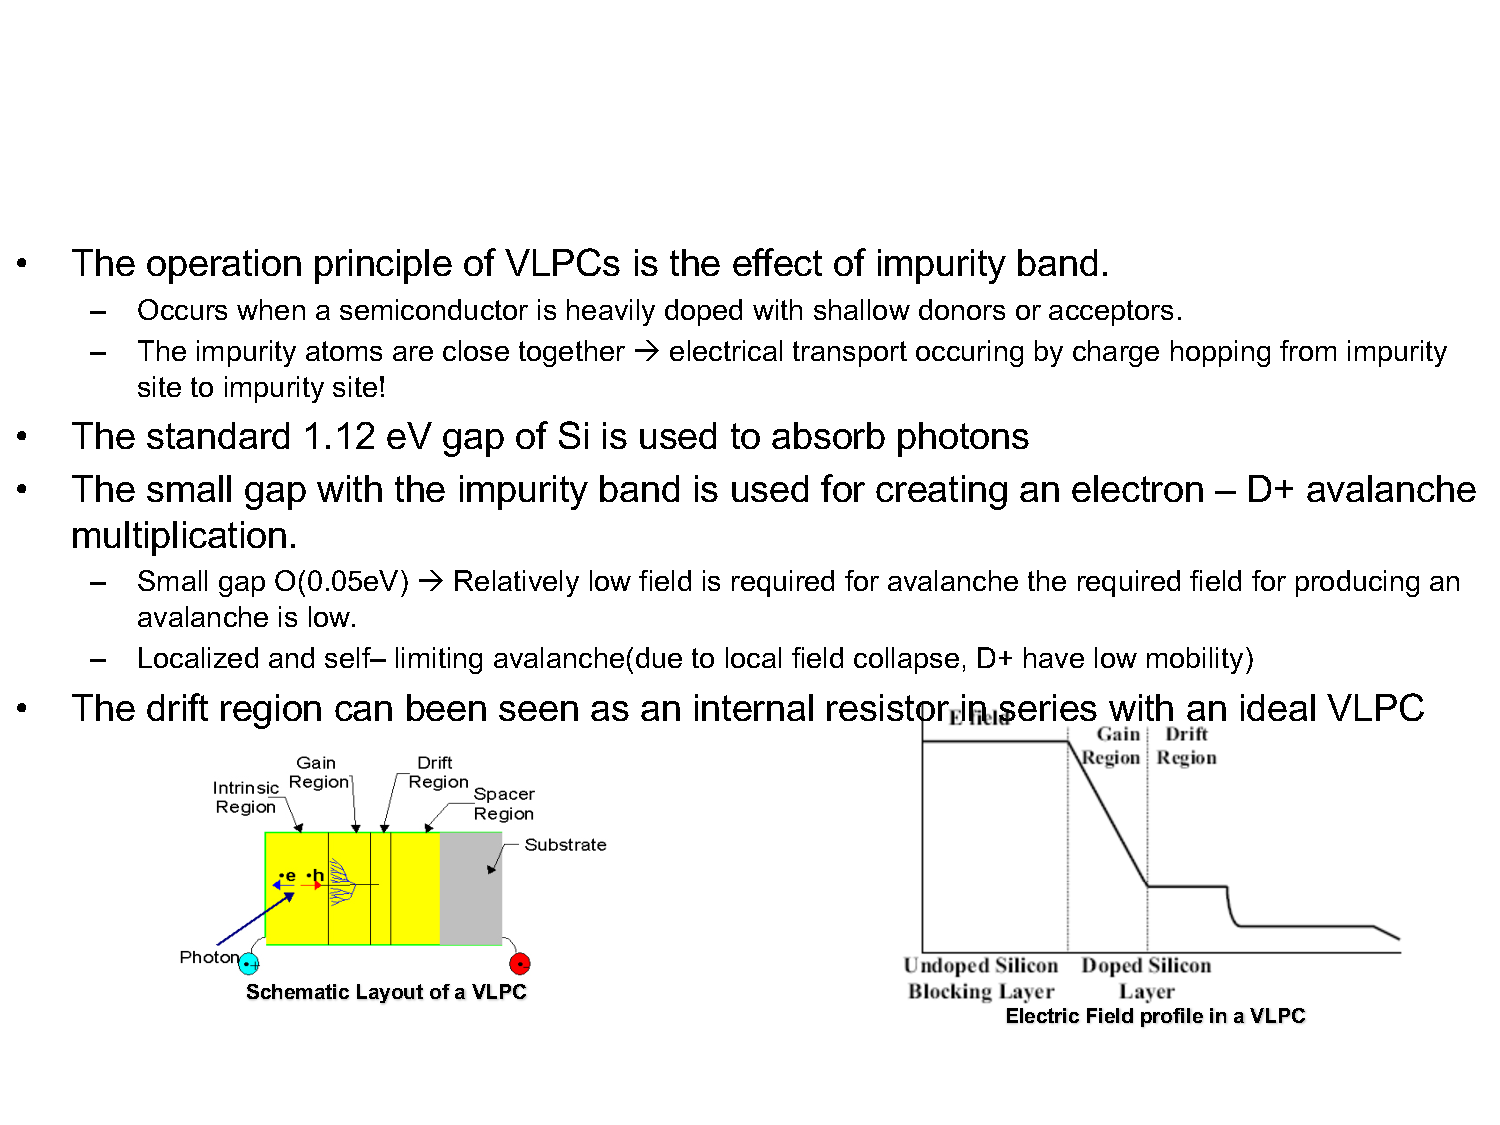
\includegraphics[width=0.95\linewidth]{./Images/107_extra_VLPCs}
  \end{figure}
\end{frame}


%%%%%% SLIDE
\begin{frame}{\textcolor{Goldenrod}{VLPCs}}
  \begin{overlayarea}{\textwidth}{\textheight}
    \begin{figure}[h]
      \centering
      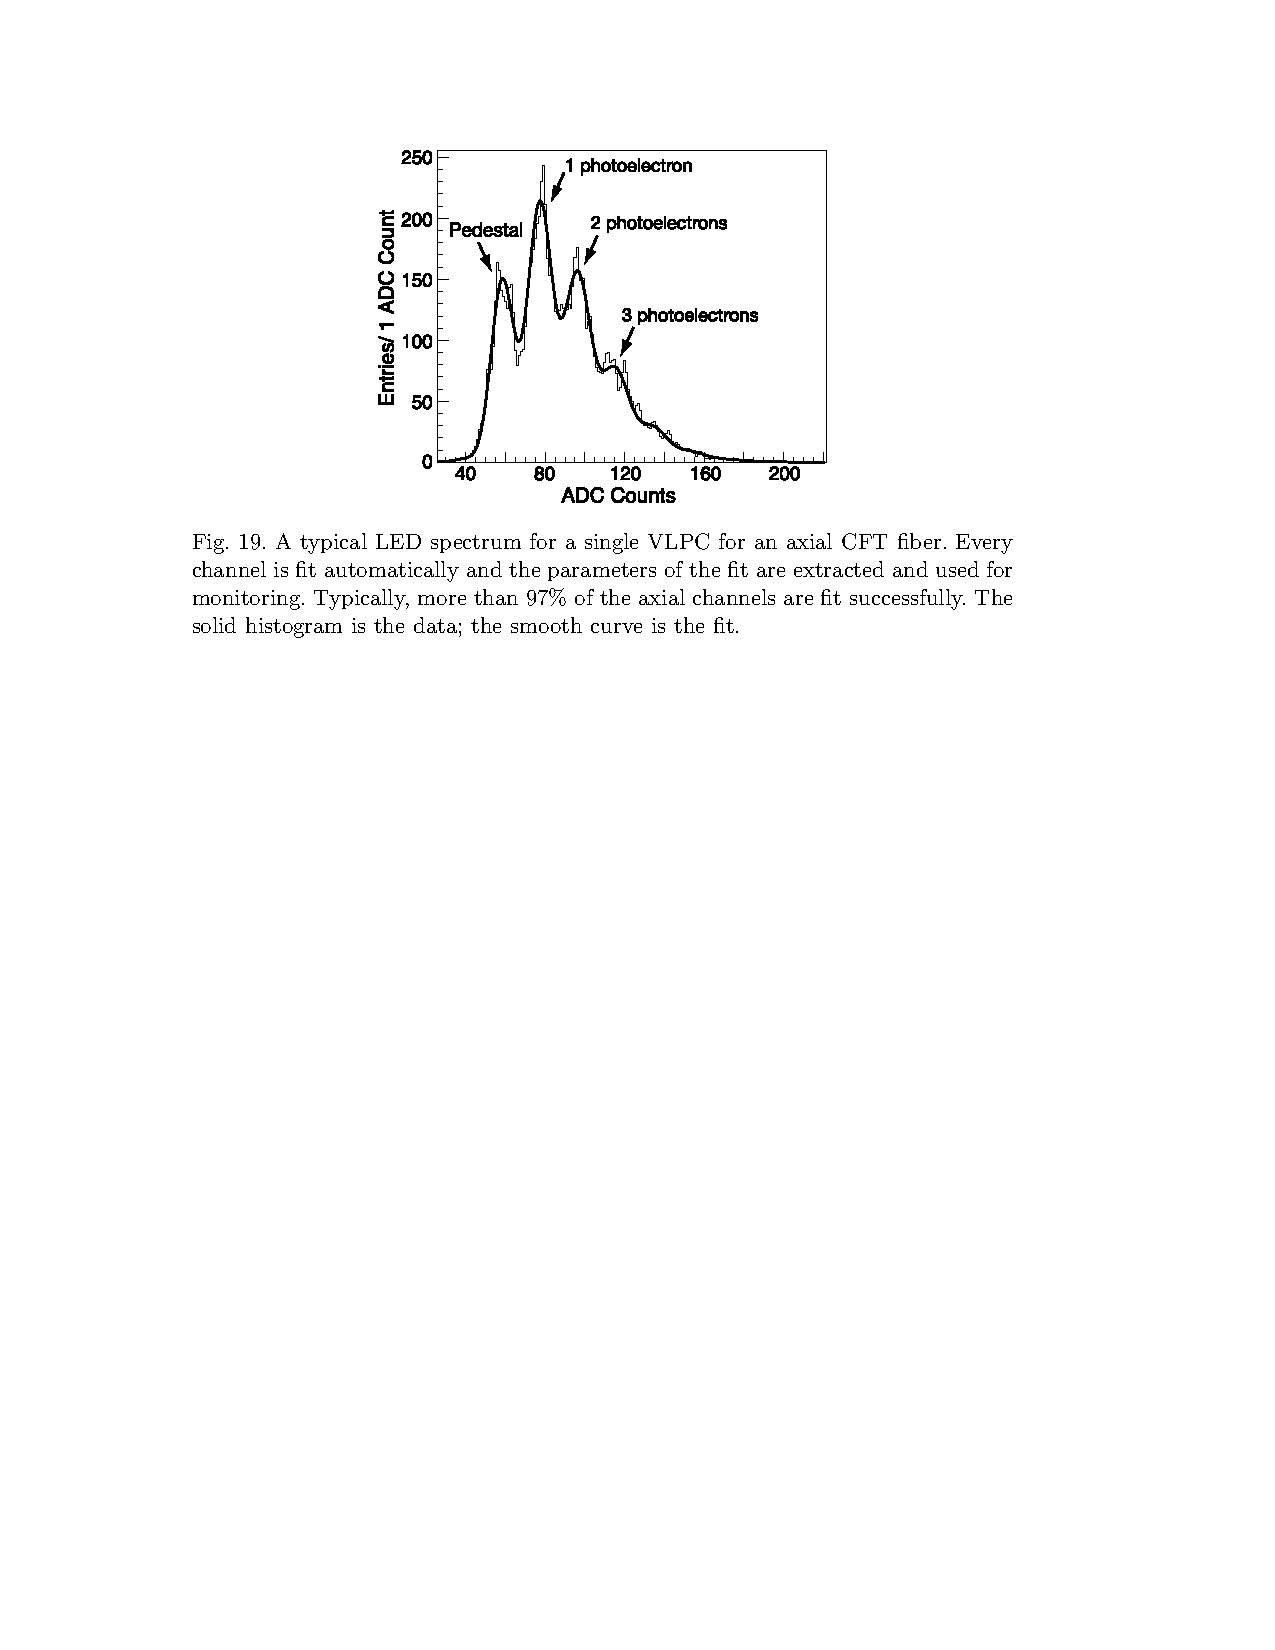
\includegraphics[width=0.8\textwidth]{./Images/109_extra_VLPCs_01}
    \end{figure}

  \end{overlayarea}
\end{frame}

%%%%%% SLIDE
\begin{frame}{\textcolor{Goldenrod}{Central Track Tigger}}
  \(
  \<{0.6\textwidth}
  \itt
\item Counts track candidates identified in axial view of CFT by
  looking for hits in all 8 axial layers
\item Combines tracking and preshower information to identify
  electron and photon candidates
\item
  Generates track lists allowing other trigger systems to
  perform track matching
  \tti
  \>
  \<{0.4\textwidth}
  \img{20_CFT}
  \>
  \)
\end{frame}



%%%%%%%%%%%%%%%%%%%%%%%%%%%%%%%%%%%%%%%%%%%%
\subsection*{Solenoidal magnet}
%%%%%% SLIDE
\begin{frame}{\textcolor{Goldenrod}{Solenoidal Magnet }}
  \(
  \<{0.45\textwidth}
  \img{26_magnet_solonoid.pdf}
  \>
  \<{0.7\textwidth}
  \itt
\item[$\Box$]<1-> to optimize the momentum resolution, $\delta p_T /p_T$ and tracking
  pattern recognition $\to $ a central field of $2 T$
\item[$\Box$]<2-> design criteria:
  \itt
\item [$i)$] to operate safely and stably at either polarity
\item [$ii)$] a uniform field over as large a percentage of the volume as practical,
\item [$iii)$] as thin as possible to make the tracking volume as large as possible,
\item [$iv)$] an overall thickness of approximately $1 X_0$ at $\eta = 0$ to optimize
  the performance of the central preshower detector mounted on the outside of
  the solenoid cryostat.
  \tti
  \tti
  \>
  \)
\end{frame}

%%%%%% SLIDE
\begin{frame}{\textcolor{Goldenrod}{Solenoidal Magnet }}
    \begin{figure}[h]
      \centering
      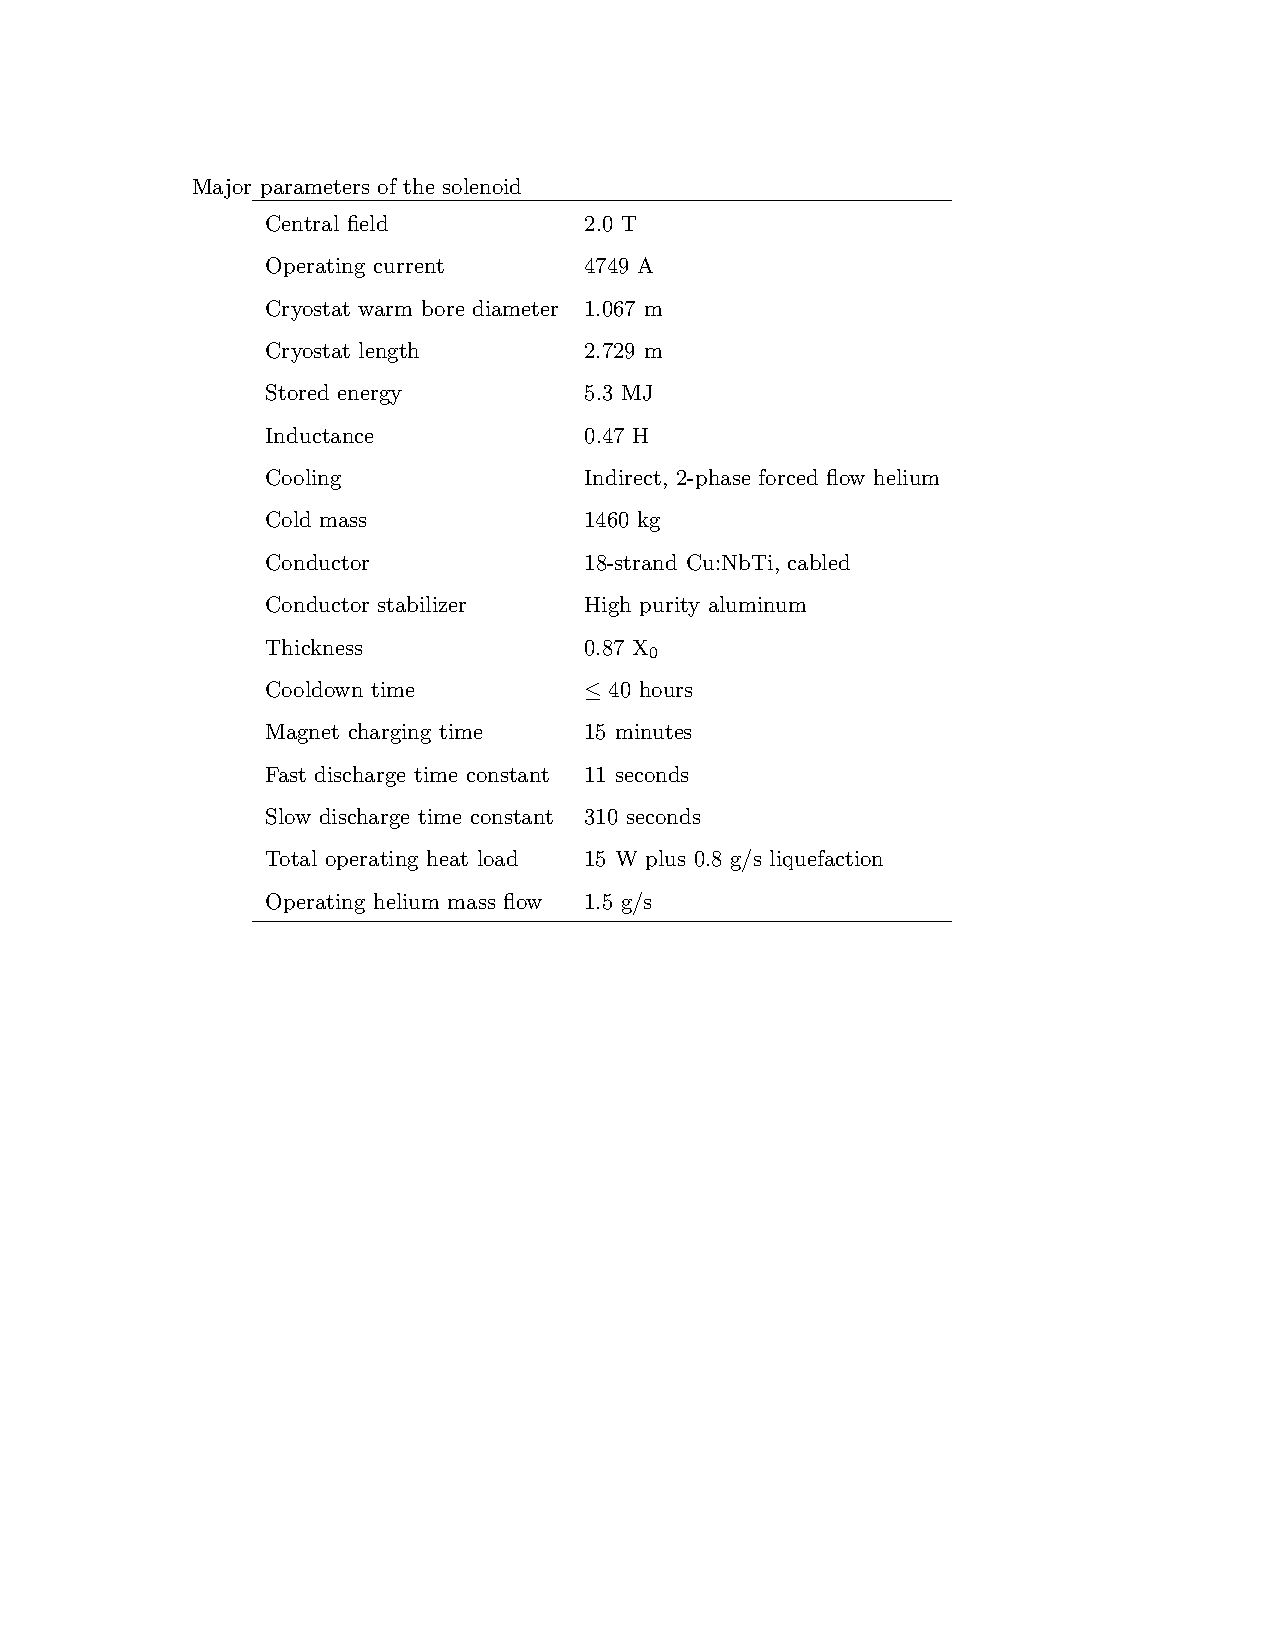
\includegraphics[height=0.6\textheight]{./Images/25_magnet_solonoid.pdf}
      \caption*{The solenoid is wound with two layers of superconductor to achieve the required
        linear current density for a $2 T$ central field.}
    \end{figure}
    
\end{frame}

%%%%%% SLIDE
\begin{frame}{\textcolor{Goldenrod}{Magnet Field}}
  \(
  \<{0.55\textwidth}
  \itt[<+->]
\item Within the solenoid (operated
  at $4749 A$), The calculated magnetic field is scaled by 0.09\%
  to agree with the measurement.
\item Within the toroid (operated at $1500 A$)
  The calculated magnetic field is scaled by $4.3\%$
  \tti
  \>
  \<{0.6\textwidth}
  \img{28_magnet_solonoid.pdf}\\
  {\scriptsize The $y-z$ view of the $D\emptyset$ magnetic field (in
    $kG$). The field
    in the central toroid is approximately $1.8 T$}
  \note{with both the toroidal
    and solenoidal magnets at full current ($1500 A$ and $4749 A$, respectively).}
  \>
  \)
\end{frame}

%%%%%%%%%%%%%%%%%%%%%%%%%%%%%%%%%%%%%%%%%%%%%%
\subsection*{Calorimetry}
%%%%%% SLIDE
\begin{frame}{\textcolor{Goldenrod}{CALO Readouts}}
  \begin{overlayarea}{\textwidth}{\textheight}
    \begin{figure}[h]
      \centering
      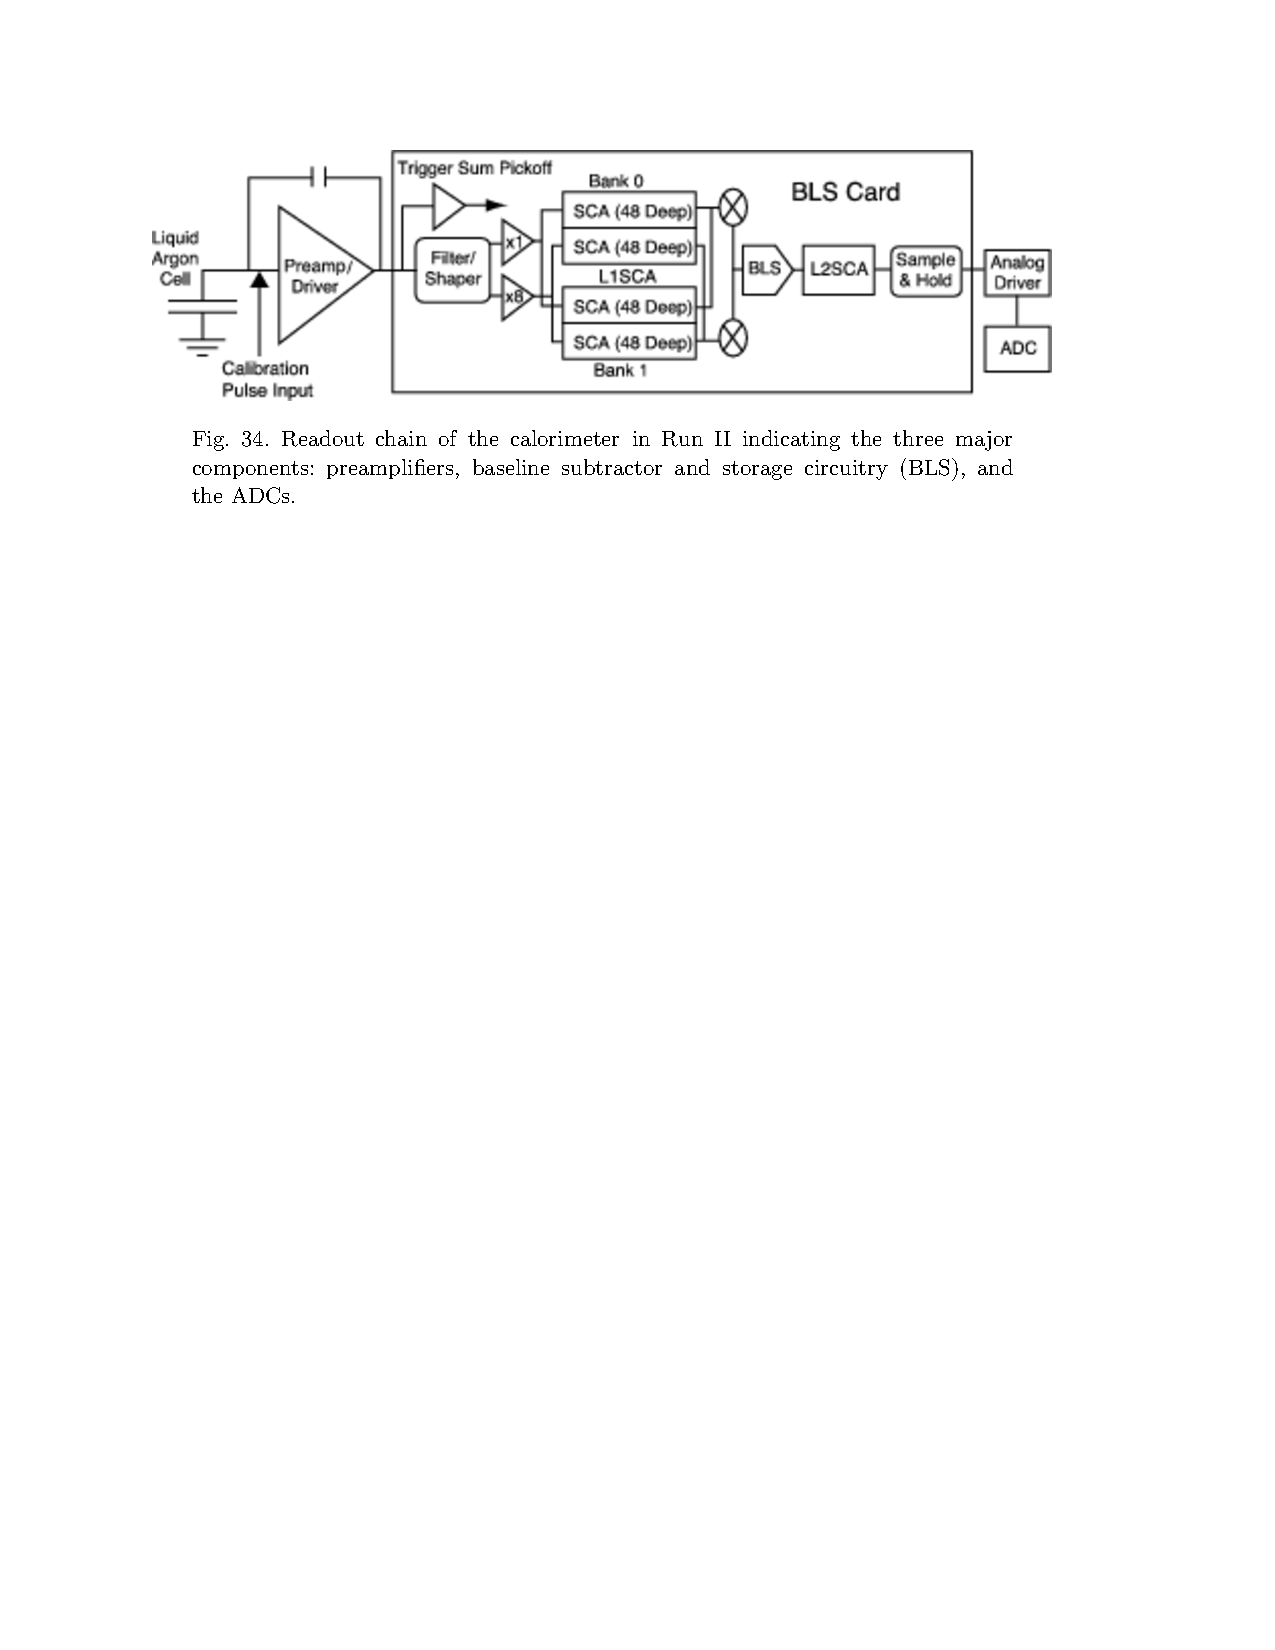
\includegraphics[width=0.8\textwidth]{./Images/110_extra_CALO_readouts}
    \end{figure}

  \end{overlayarea}
\end{frame}


%%%%%%%%%%%%%%%%%%%%%%%%%%%%%%%%%%%%%%%%%%%%%%
\subsection*{Muon detector}
%%%%%% SLIDE
\begin{frame}{\textcolor{Goldenrod}{Muon Tracking System }}
  \begin{overlayarea}{\textwidth}{\textheight}
    \begin{figure}[h]
      \centering
      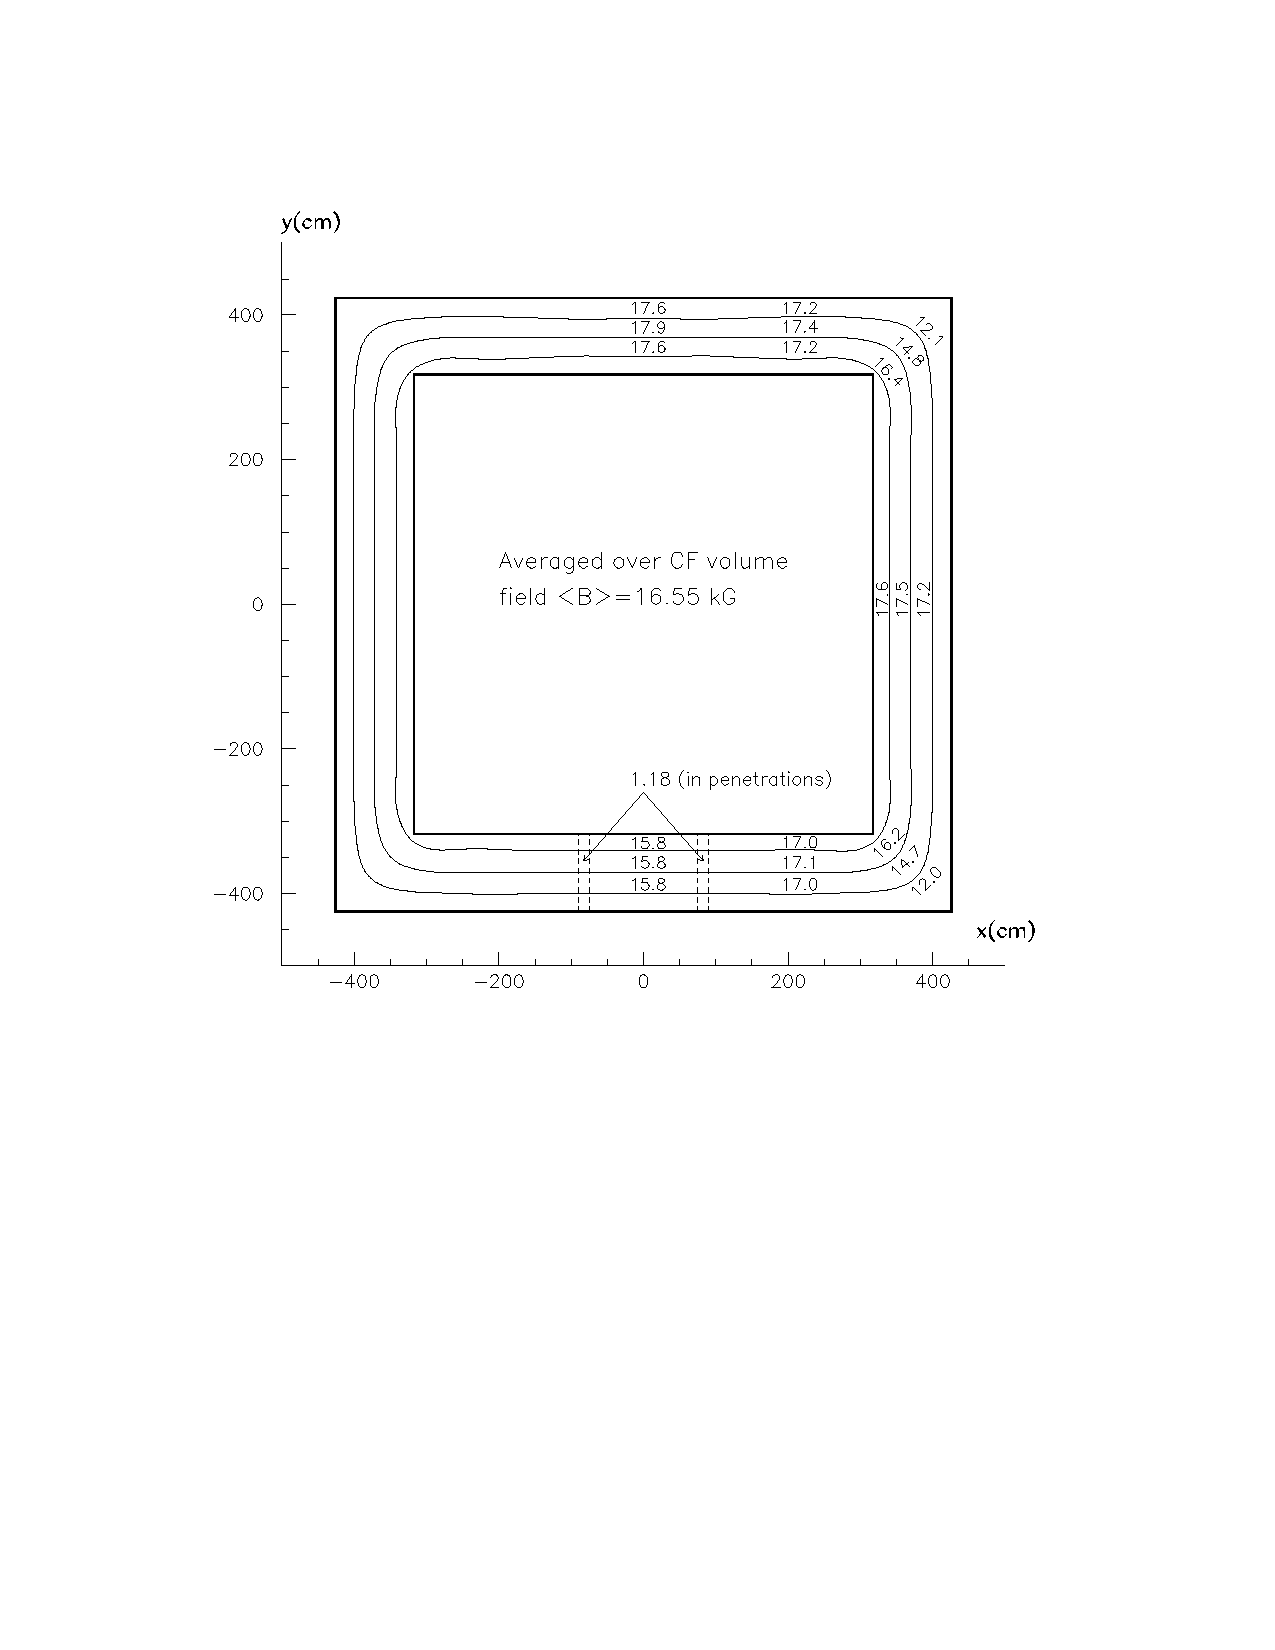
\includegraphics[height=0.7\textheight]{./Images/42_MD_central_magnet}
      \caption*{{\scriptsize Magnetic field in the central toroid
          magnet. The magnetic field is in $kG$.}}
    \end{figure}

  \end{overlayarea}
\end{frame}


%%%%%% SLIDE
\begin{frame}{\textcolor{Goldenrod}{Combinatorial Background}}
  \begin{overlayarea}{\textwidth}{\textheight}
    \begin{figure}[h]
      \centering
      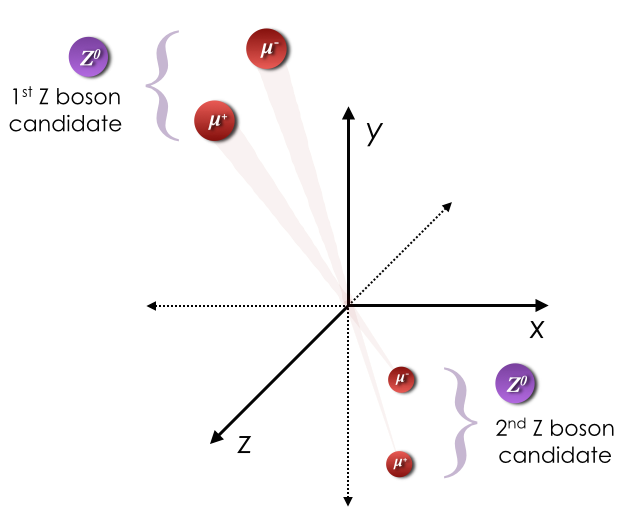
\includegraphics[height=0.5\textheight, width=0.5\textwidth]{./Images/103_extra_combinatorial_bkgs_01}
      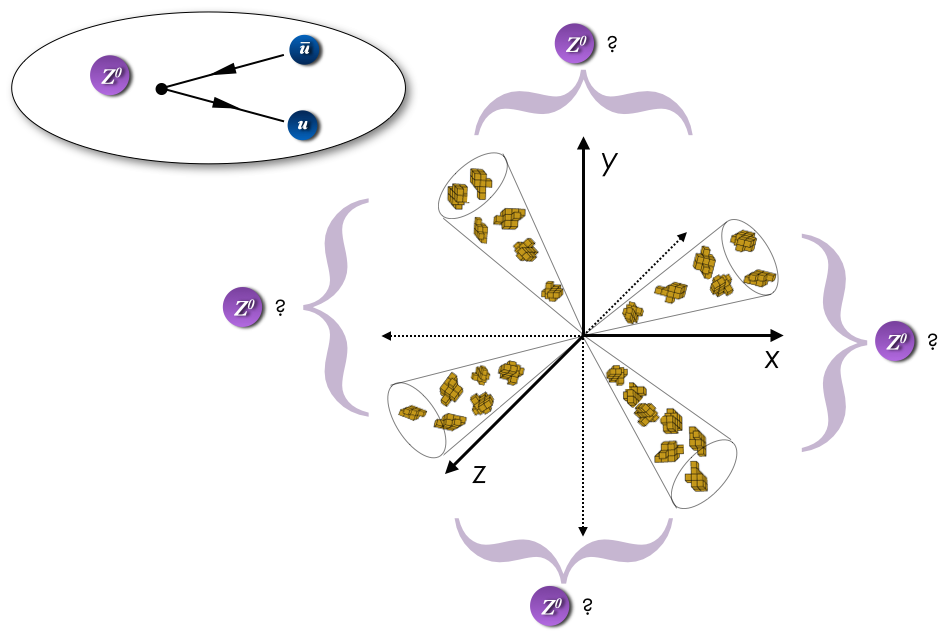
\includegraphics[height=0.5\textheight, width=0.5\textwidth]{./Images/103_extra_combinatorial_bkgs_02}
    \end{figure}
    
    \itt
  \item the non-background background!
    \tti
  \end{overlayarea}
\end{frame}


%109_extra_VLPCs_01
%110_extra_CALO_readouts

%%%%%% SLIDE
\begin{frame}{\textcolor{Goldenrod}{Differential Signaling}}
  \begin{overlayarea}{\textwidth}{\textheight}
    \begin{figure}[h]
      \centering
      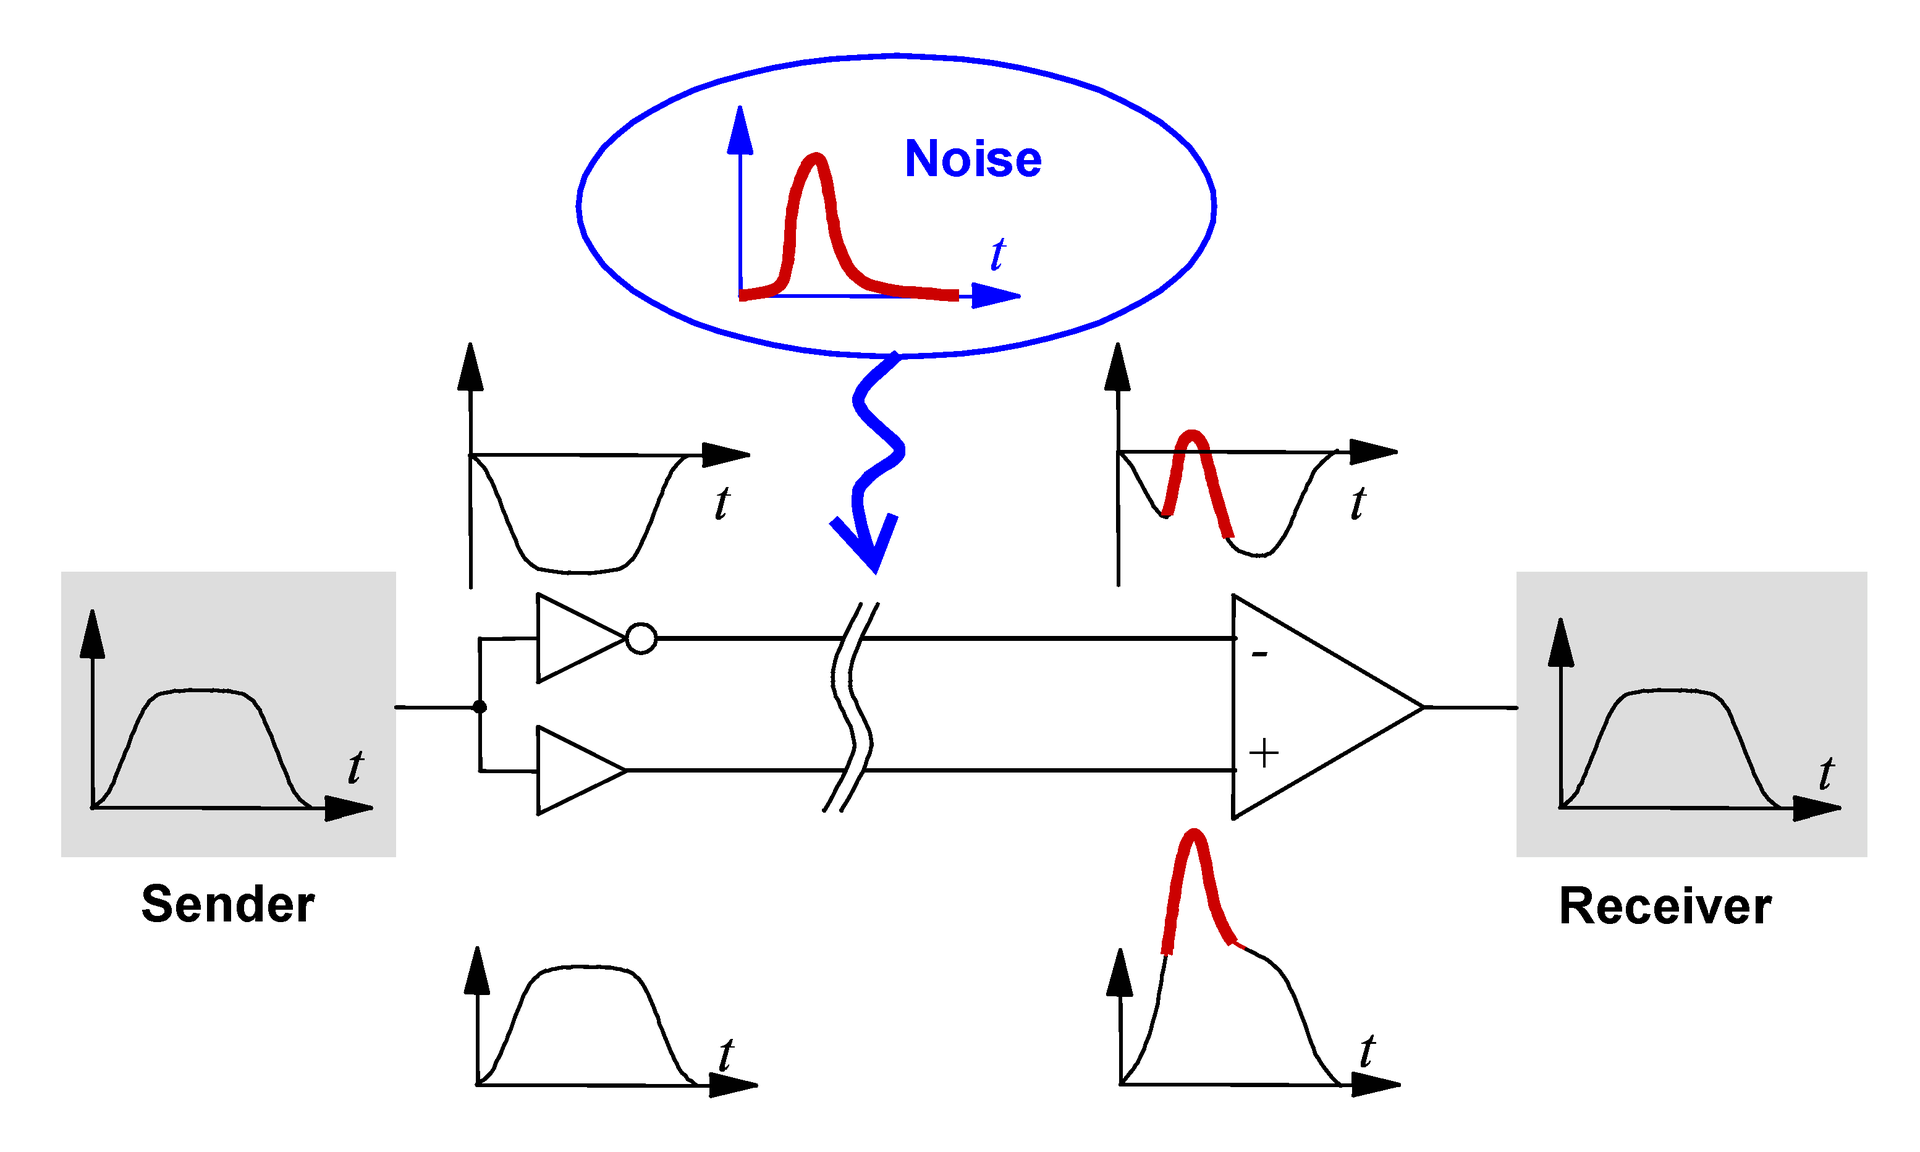
\includegraphics[width=0.8\textwidth]{./Images/108_extra_DiffSignaling}
    \end{figure}
    
  \end{overlayarea}
\end{frame}


\backupend
\end{document}



%%%% frame template
%%%%%%%%% SLIDE
% \begin{frame}{\textcolor{Goldenrod}{Title }}
%   \begin{figure} \centering
%     %%%% figure manipulation 
%     \begin{tikzpicture}[zoomboxarray,connect zoomboxes, zoombox paths/.append style={ultra thick, red}]
%       \node [image node, help grid]
%       { 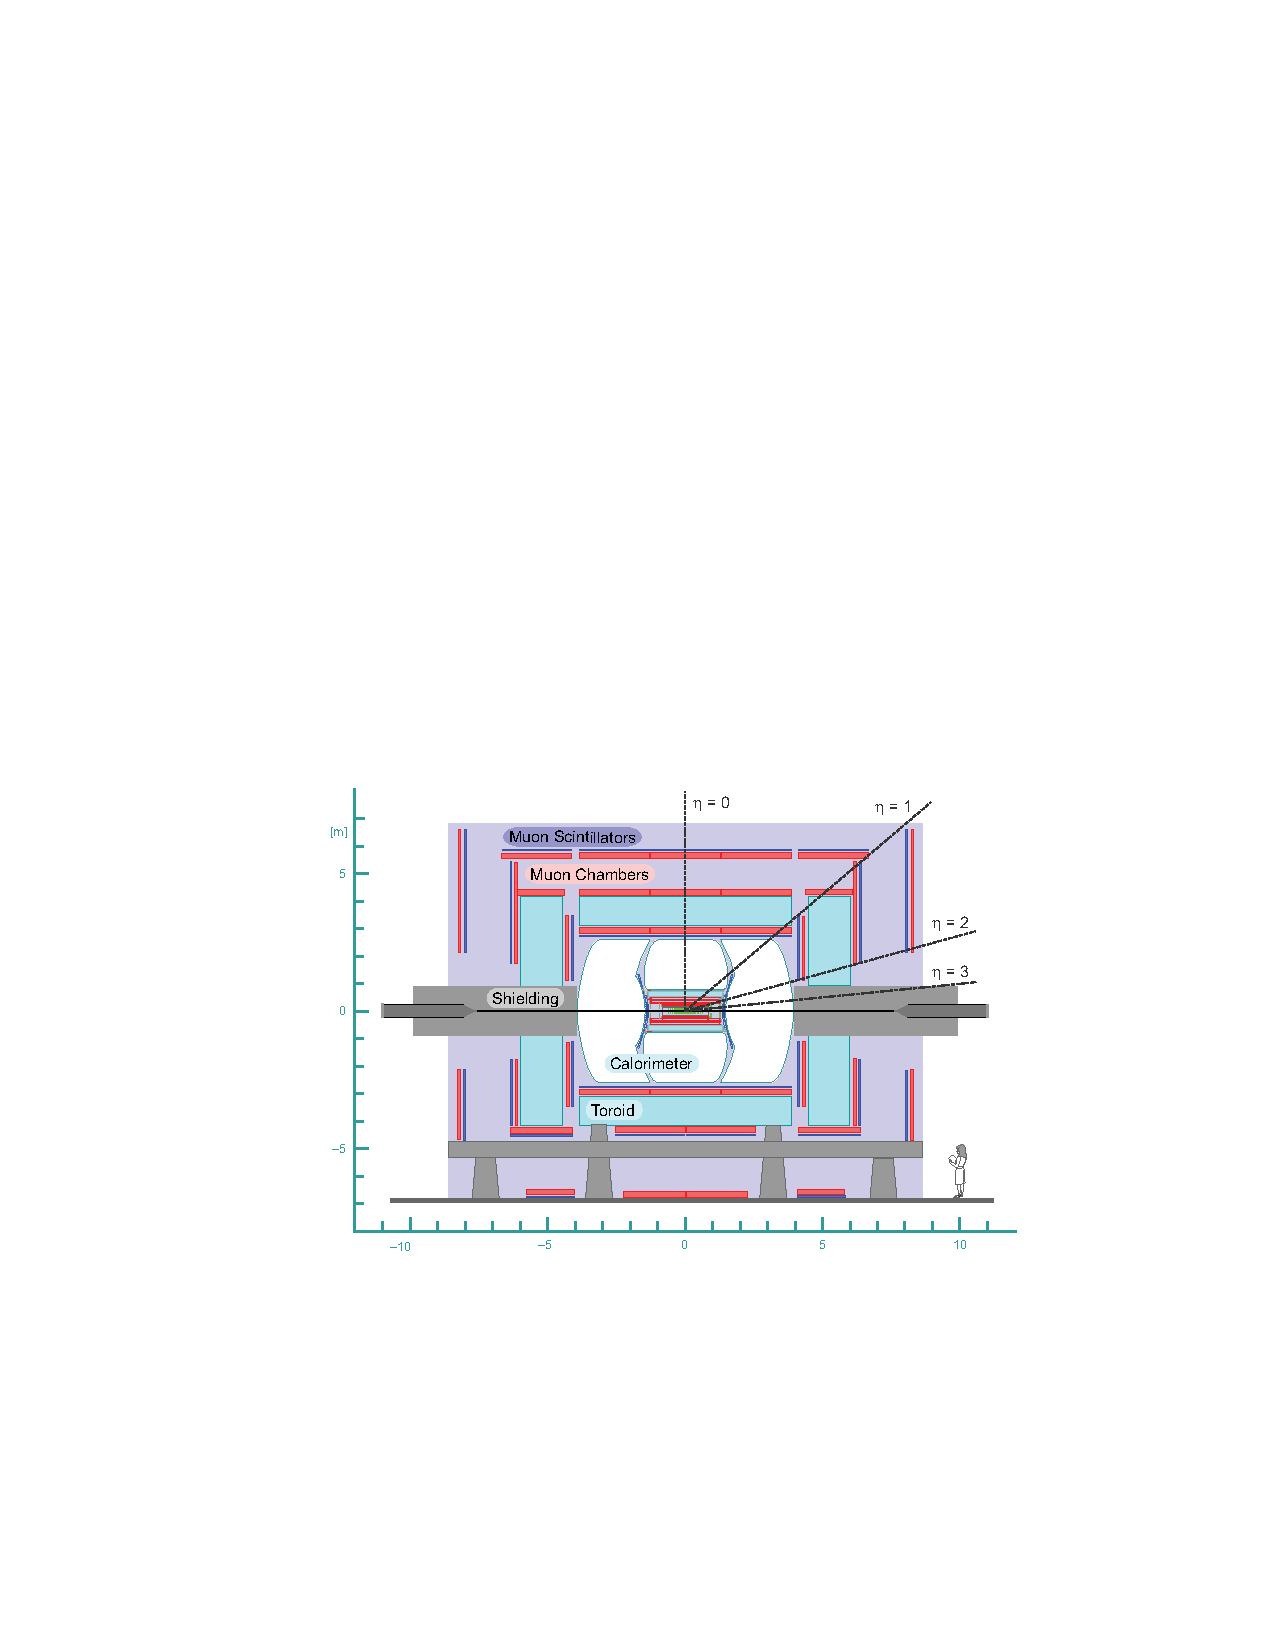
\includegraphics[width=0.45\textwidth]{./Images/01_dzero_wholedetector.pdf}};
%       \onslide<2->\zoombox[magnification=5,color code=lime]{0.86,0.35}
%     \end{tikzpicture}
%   \end{figure}
% \end{frame}
